% Chapter 3
\chapter{بررسی پیشینه روش‌های حل مشکل ناهمگنی آماری}

\section{مقدمه}
همان‌طور که در فصل گذشته اشاره شد، یکی از مهم‌ترین مشکلات در حوزه یادگیری فدرال، مسئله داده‌های غیرمستقل و غیریکنواخت
\lr{(non-IID)}
است که منجر به بروز چالش‌ها و ناهمگنی‌های آماری می‌شود. این مشکل باعث می‌شود که مدل‌های یادگیری نتوانند به خوبی از داده‌های توزیع‌شده استفاده کنند و کارایی مطلوبی داشته باشند. به دلیل اهمیت بالای این موضوع، محققان بسیاری تلاش‌های گسترده‌ای برای حل این مشکل انجام داده‌اند.

مبحث اصلی این پایان‌نامه نیز به طور دقیق به همین مسئله اشاره دارد و به دنبال یافتن راه‌حلی مؤثر برای مقابله با داده‌های
\lr{non-IID}
است. در ادامه، به صورت خلاصه به بررسی راه‌حل‌هایی که تاکنون برای حل این مشکل مطرح شده‌اند، خواهیم پرداخت تا تصویر جامعی از تلاش‌های انجام شده در این زمینه ارائه دهیم. همچنین باید توجه داشت که هر یک از این راه‌حل‌ها نقاط قوت و ضعف خاص خود را دارند و بسته به شرایط و نوع داده‌ها، می‌توانند نتایج متفاوتی را به همراه داشته باشند. بررسی دقیق این راه‌حل‌ها و ارزیابی کارایی آن‌ها می‌تواند به بهبود سیستم‌های یادگیری فدرال و غلبه بر مشکلات مرتبط با داده‌های غیرمستقل و غیر یکنواخت کمک شایانی کند.

\section{نگرش برپایه داده}
\subsection{اشتراک‌گذاری داده}
مشکل اصلی الگوریتم
\lr{FedAvg}
در مواجهه با داده‌های غیرمستقل و غیریکنواخت، تفاوت وزن‌های اولیه در شروع فرآیند آموزش است. این تفاوت‌ها می‌توانند باعث شوند که مدل‌های محلی در هر گره به طور قابل توجهی متفاوت از یکدیگر باشند، که در نتیجه منجر به مشکلات همگرایی و کاهش کارایی مدل نهایی می‌شود.

برای رفع این مشکل، روشی پیشنهاد شده است که در آن ابتدا سرور مرکزی مقدار کمی از داده‌ها را به صورت محلی آموزش می‌دهد. در این مرحله، سرور مرکزی با استفاده از این داده‌ها، یک مدل اولیه را آموزش داده و وزن‌های اولیه آن را تنظیم می‌کند. سپس، این وزن‌های اولیه به همراه داده‌های آموزش دیده به تمامی کاربران ارسال می‌شود. این اقدام باعث می‌شود که تمام کاربران در ابتدای فرآیند آموزش با مجموعه‌ای از داده‌های مشترک و وزن‌های اولیه مشابه روبه‌رو شوند.

نقطه قوت این روش در این است که به دلیل انجام این عملیات تنها در آغاز فرآیند آموزش، هزینه زیادی به شبکه تحمیل نمی‌شود. در واقع، انتقال داده‌ها و وزن‌ها فقط در ابتدا انجام شده و پس از آن کاربران به صورت مستقل به آموزش مدل‌های محلی خود ادامه می‌دهند. این اقدام منجر به کاهش اختلافات ناشی از ناهمگونی داده‌ها شده و فرآیند همگرایی مدل نهایی سریع‌تر و با دقت بیشتری انجام می‌شود
\cite{zhao2018federated}.

در شکل
\ref{share_data}%
، نحوه اجرای این روش و مراحل مختلف آن به تصویر کشیده شده است. این تصویر نشان می‌دهد که چگونه سرور مرکزی ابتدا داده‌های کمی را آموزش می‌دهد، وزن‌های اولیه را تنظیم می‌کند و سپس این وزن‌ها و داده‌ها را به کاربران ارسال می‌کند تا فرآیند آموزش محلی با یک نقطه شروع مشترک برای همه کاربران آغاز شود.

 \begin{figure}[t]
	\centering
	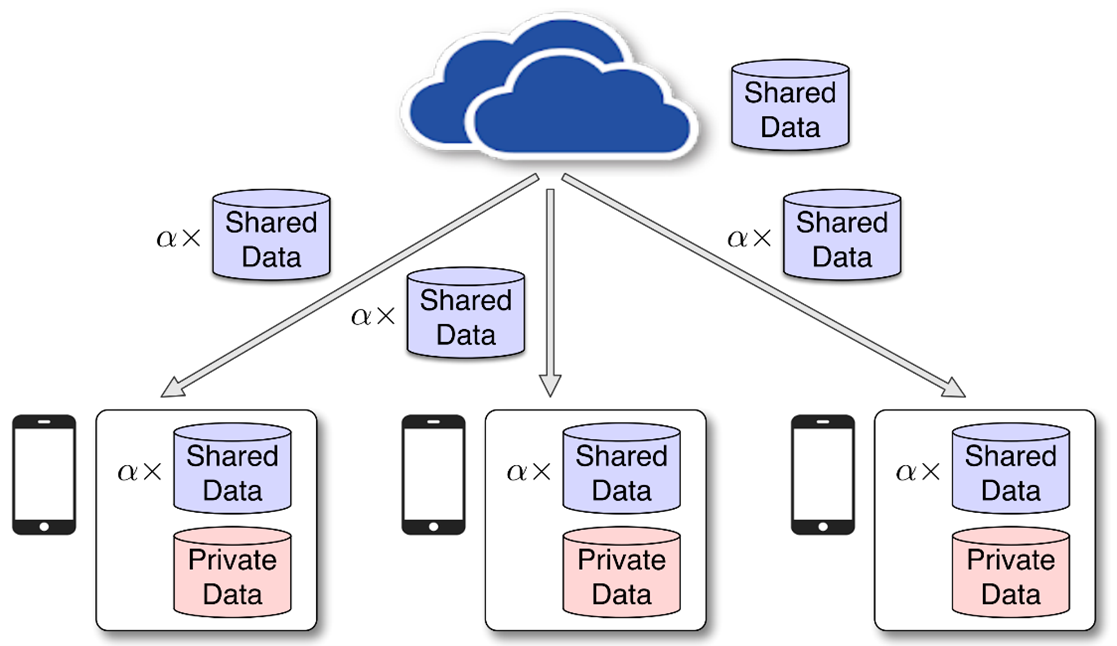
\includegraphics[scale=0.9]{images/chap3/share_data.png}%
	\caption{%
		نمایش نحوه به اشتراک‌ گذاری داده
		\cite{zhao2018federated}%
		.
	}
	\label{share_data}
	\centering
\end{figure}

%یک روش بیان شده دیگر به این نحو است که کاربران بتوانند نتیجه آموزش تعدادی داده اشتراکی را برای یکدیگر ارسال کرده و از نتایج دیگر کاربران بر روی داده‌های اشتراکی اطلاع داشته باشند [32]. با توجه به بررسـی‌های انجام گرفته برای مثال، بر روی مجـموعه‌داده CIFAR-10 اگر حـدود 5درصد داده‌ها به صـورت اشتراکی در اختیار کاربران قرار گیرد، دقت مدل حدود 30درصد افزایش خواهد یافت. البته ذکر این نکته خالی از لطف نیست که روش به اشتراک‌گذاری داده‌ها بین کاربران، خود می‌تواند باعث نقض حریم شخصی شود و هنگام پیاده‌سازی این روش باید موارد مورد نیاز جهت حفظ حریم شخصی کاربران به صورت جدی مورد بررسی قرار گیرد [33].


\subsection{تست}
تست

\subsection{تست}
تست



\section{نگرش برپایه مدل}
تست


\section{نگرش برپایه چهارچوب}
تست


\section{نگرش برپایه الگوریتم}
تست
